\documentclass{ee208report}

\title{Lab Report 13}

\begin{document}

\begin{CJK}{UTF8}{gbsn}
    \maketitle
\end{CJK}

\begin{multicols*}{2}

\section{Introduction}

In this lab report, we present our implementation of a Locality Sensitive Hash
(LHS) table, which enables fast query of an image in an image database.

The report is organized as follows: The idea and implementation of LHS are
interleaved in the following sections to give an outline of the LHS algorithm
and our implementation. Then, the performance of the hash table is measured
under various parameters, such as the map sets used for LHS and the number of
nearest neighbors to return. The LHS table is also put to test with an ORB-based
nearest neighbor image search to compare search results.

\begin{figure}[H]
    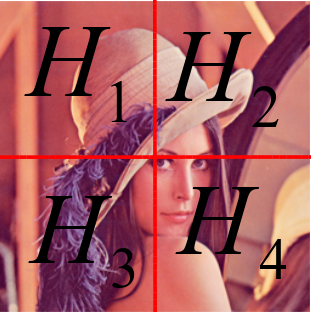
\includegraphics[width=\linewidth]{images/4_regions.png}
    \caption{An image divided into 4 regions for generating feature vectors}
    \label{fig:regions}
\end{figure}

\section{Generating Feature Vectors}

The LSH function only accepts vectors with integer components as input, so each
image must be converted to a vector. In our implementation, the function
\texttt{feature\_vector()} converts an image into a vector. An input image is
evenly divided into 4 regions, and color histograms are calculated for each
region, as shown in Figure~\ref{fig:regions}. 

The histograms for the 4 regions are concatenated to form a 12-dimensional
vector. For each component of the vector, if the component is less than 0.3, it
is assigned the value 0, or else it is assigned the value 1 if the component is
not less than 0.3 but less than 0.6. Otherwise, that component is assigned 2.
The implementation of \texttt{feature\_vector()} is available in
Listing~\ref{lst:feature-vector}.

\section{The LSH Function}

The Locality Sensitive Hash function, implemented as \texttt{lsh()}, returns an
integer (in its binary representation) like any other hash functions. In this
lab report, we take the approach of bit sampling over unary coding.

\subsection{Unary coding}

Unary coding encodes an integer $n$ into a binary with code length $C$ ($n \leq
C$). The binary consists of $n$ 1s and $(C - n)$ 0s. For example, the integer 3
will be converted to 11100 under unary coding with code length $C = 5$.

To encode a vector with integer components in unary code, each component is
individually encoded in unary code and then encoded binaries are concatenated,
so the vector (2, 3, 4, 5) will be encoded as 11000 11100 11110 11111 (spaces
inserted for clarity) with code length 5.

\subsection{Bit sampling}

We define the result of bit-sampling of a binary over a set $I \subset
\mathbb{Z_{++}}$ to be a binary. The binary is formed as follows: For each
element $x \in I$, we take $x$th bit of the binary in a left-to-right fashion.
As a final example, sample the binary 11000 11100 11110 11111 over the set \{2,
9, 12, 18\} yielding the binary 1011.

\subsection{LHS}

The LHS function works by first encoding a vector in unary coding and then
bit-sampled the binary over a set $I$. Note that different sets for bit-sampling
correspond to different hash functions. Actually, to find the hash value for a
vector, there is no need to unary-encode a vector. If we divide an encoded
vector $v$ (components denoted by $v_i$) into segments of length $C$, where $C$
is the code length for unary coding, then each segment corresponds to the a
component of the original vector. To bit-sample the vector, we select, say,
$k$th bit of the encoded binary. If the $k$th bit falls in the $j$th segment,
which implies $(j - 1)C < k \leq jC$, then the $k$th bit is 1 if $k - (j - 1)C
\leq v_i$ and 0 otherwise.

To see why this is the case, here is an example. Again, the vector is (2, 3, 4,
5) and the encoded version is 11000 11100 11110 11111 for $C = 5$. Since each
segment in the binary begins with a series of 1s, to sample the $k$th bit, where
$k = 12$, we want to know which segment the 12th bit falls in --- that's the 3rd
segment. Instead of directly looking at the 12th bit, we look at the second bit
of the third segment. We know the 12th bit is the second bit of the third
segment because

\[
    k - (j - 1)C = 2
\]

where $k = 12, j = 3, C = 5$. Now that $2 \leq v_3 = 4$, the third segment begin
with four 1s, so the second bit in the third segment is clearly 1. To express
such idea of the $j$th segment, we partition a set $I$ into $I|1, I|2,\dots,
I|n$, where $n$ is the length of the original vector, and define

\[
    I|j = \{k \in I|(j - 1)C < k \leq jC\}
\]

In this way, $I|j$ contains all such $k \in I$ that falls in the $j$th segment
of the unary code. In our implementation in Listing~\ref{lst:lsh}, we go one
step further because the function \texttt{lsh()} takes as input a vector and a
segmented map set. A segmented map set $I'$ is

\[
    I' = \{I'|j|j = 1, 2,\dots, n\}
\]

where

\[
    I'|j = \{k - (j - 1)C|(j - 1)C < k \leq jC, k \in I\}
\]

A segmented version of $I$ allows fast computation of LSH. The final result of
LSH is a binary and is converted to a decimal.

\section{LSH Table}

LSH Table is a hash table that uses LSH as the sole hash function. It is
implemented as the class \texttt{LSHTable} with three methods:

\begin{description}
    \item[\texttt{segment\_map\_set()}] Segment $I$ to generate $I'$;
    \item[\texttt{add()}] Add a vector and associated satellite data (in our
    case, filename of an image) to the table for later query;
    \item[\texttt{knn()}] Find $k$ nearest neighbors. Distances are measured in
    Euclidean distance.
\end{description}

\texttt{knn()} may need further elaboration. Devising new LSH functions are easy
because a different map set gives a different hash function. There are more than
one hash functions for \texttt{LSHTable}. When finding $k$ nearest neighbors,
first a list of candidates is drawn from vectors that are hashed to the same
value as the input vector for each hash function. To determine similarity
between a candidate and the input vector, their Euclidean distance is
calculated. The code is available in the file \texttt{lsh\_demo.py}.

\section{Performance}

\subsection{KNN}

We take an alternative approach to find KNN for an input image as a comparison.
This implementation is based on ORB and brute-force matcher. We extract ORB
descriptors from each image in the dataset and match them against the target
image with the brute-force matcher. Distances between two images are defined as
the sum of distance between two descriptors in each pair of the 10 best-matched
descriptor pairs.

There could be alternative definition of distance, though. One idea is to devise
a threshold so that a matched descriptor is accepted if and only if the distance
between the two is less than the threshold. The distance between two images will
be the number of accepted descriptor pairs. But we found out that some images so
distinct from the target that the distance in most of the descriptor pairs shows
little variation. An arbitrary threshold will definitely accept some of the
pairs while reject the rest even if their distances are similar. Therefore, this
approach is not implemented.

The KNN implementation is available in Listing~\ref{lst:knn}. 8 nearest
neighbors are found as an example.

We measure the performance of our KNN implementation when finding 8 nearest
neighbors with the bash keyword \texttt{time}. It measures on average 0.432
seconds, including time for extracting descriptors and matching.

\subsection{Variation on the length of map set}

We instruct the LSH table to return 8 nearest neighbors for the target image.
The LSH table has 5 map sets. The map sets with length 15 are constructed from
the map sets with length 20 by removing the last element of every 4 element.
Similarly, the map sets with length 10 are constructed from the map sets with
length 15 by removing the last element of every 3 element. The original map sets
with length 20 are shown in Listing~\ref{lst:testing-data} and results are
available in Table~\ref{tbl:time-by-length}.

\begin{table}[H]
    \centering
    \begin{tabular}{r r}
        \toprule
        Length of map set & Running time/s \\
        \midrule
        20 & 0.218 \\
        15 & 0.221 \\
        10 & 0.220 \\
        5 & 0.214 \\
        \bottomrule
    \end{tabular}
    \caption{Running time by length}
    \label{tbl:time-by-length}
\end{table}

\subsection{Variation on the number of map sets}

Again, we instruct the LSH table to return 8 nearest neighbors. The LSH table
may have 8, 5 or 2 map sets, where the 5 map sets are constructed by deleting
the last 3 map sets from the 8 map sets, and the 2 map sets are constructed by
deleting the last 3 map sets from the 5 map sets. The original 8 map sets are
shown in Listing~\ref{lst:testing-data} and results are shown in
Table~\ref{tbl:time-by-number}.

\begin{table}[H]
    \centering
    \begin{tabular}{r r }
        \toprule
        Number of map sets & Running time/s \\
        \midrule
        8 & 0.231 \\
        5 & 0.223 \\
        2 & 0.238 \\
        \bottomrule
    \end{tabular}
    \caption{Running time by number of map sets}
    \label{tbl:time-by-number}
\end{table}

\section{Conclusion}

In our test, the LSH-based nearest neighbor search beats ORB-based nearest
neighbor search by a wide margin. And variation on the map sets (number and
length) doesn't make a conceivable difference on the running time of the nearest
neighbor search.

\end{multicols*}

\begin{listing}
    \begin{minted}[frame=lines, linenos]{python}
def feature_vector(img):
    half_height = img.shape[0] // 2
    half_width = img.shape[1] // 2
    # divide into 4 regions
    regions = (img[:half_height, :half_width], img[:half_height, half_width:],
               img[half_height:, :half_width], img[half_height:, half_width:])
    hists = []
    for r in regions:
        # sum of intensity of each color
        hist = np.array([r[:, :, i].sum() for i in range(3)], np.float64)
        hists.append(hist / hist.sum())
    v = np.concatenate(hists)
    for i in range(v.shape[0]):
        if v[i] < 0.3:
            v[i] = 0
        elif v[i] < 0.6:
            v[i] = 1
        else:
            v[i] = 2
    return v.astype(np.uint8)
    \end{minted}
    \caption{The function for converting an image to a vector}
    \label{lst:feature-vector}
\end{listing}

\begin{listing}
    \begin{minted}[frame=lines, linenos]{python}
def lsh(v, seg_map_set):
    """
    Locality Sensitive Hashing
    :param v: vector
    :param seg_map_set: segmented map set
    :return: int
    """
    result = ''
    for i, s in enumerate(seg_map_set):
        if len(s):
            # count elements in s that are less than v[i]
            count = 0
            for x in s:
                if x <= v[i]:
                    count += 1
                else:
                    break
            result += '1' * count + '0' * (len(s) - count)
    # represent the hash value as a decimal
    return int(result, 2)
    \end{minted}
    \caption{LSH function}
    \label{lst:lsh}
\end{listing}

\begin{listing}
    \begin{minted}[frame=lines, linenos]{python}
import cv2 as cv

if __name__ == '__main__':
    orb = cv.ORB_create()
    bf = cv.BFMatcher(cv.NORM_HAMMING, crossCheck=True)
    target = cv.imread('target.jpg')
    # preserve descriptors but discard keypoints
    _, target_des = orb.detectAndCompute(target, None)
    
    directory = 'Dataset/'
    dataset = []
    for i in range(1, 41):
        filename = str(i) + '.jpg'
        img = cv.imread(directory + filename)
        _, des = orb.detectAndCompute(img, None)
        matches = bf.match(des, target_des)
        # sort matches in the order of their distance
        matches.sort(key=lambda x: x.distance)
        
        # sum the distances of the 10 closest matches
        sum_of_distance = 0
        for j in range(5):
            sum_of_distance += matches[j].distance
        # each element in dataset is a tuple with format
        # (filename, sum of distance)
        dataset.append((filename, sum_of_distance))
    
    dataset.sort(key=lambda x: x[1])
    print(dataset[:8])
    \end{minted}
    \caption{KNN with ORB features}
    \label{lst:knn}
\end{listing}

\begin{listing}
    \begin{minted}[frame=lines, linenos]{python}
# the map sets of length 20 used for testing LSH with different map set length
map_set1 = [
    [1, 2, 3, 4, 5, 6, 7, 8, 9, 10, 11, 12, 14, 15, 16, 18, 19, 20, 22, 23],
    [1, 2, 3, 4, 5, 6, 9, 10, 11, 12, 13, 15, 16, 17, 18, 20, 21, 22, 23, 24],
    [1, 2, 3, 4, 5, 6, 8, 9, 10, 11, 12, 13, 14, 16, 19, 20, 21, 22, 23, 24],
    [1, 2, 3, 4, 5, 8, 9, 10, 11, 12, 13, 14, 15, 16, 17, 18, 19, 20, 22, 23],
    [1, 2, 5, 6, 7, 8, 9, 10, 11, 12, 13, 14, 15, 16, 18, 19, 20, 21, 23, 24]
]
# 8 map sets used for testing LSH with different number of map sets
map_set2 = [
    [3, 4, 5, 6, 7, 9, 10, 15, 21, 23],
    [1, 3, 8, 10, 12, 13, 16, 18, 21, 22],
    [1, 4, 6, 8, 11, 12, 15, 16, 17, 22],
    [1, 2, 3, 5, 7, 9, 11, 16, 17, 19],
    [1, 2, 6, 8, 9, 12, 14, 20, 21, 22],
    [2, 5, 7, 8, 12, 13, 14, 15, 18, 23],
    [1, 2, 5, 14, 17, 19, 20, 22, 23, 24],
    [1, 2, 5, 8, 11, 12, 14, 16, 17, 18]
]
    \end{minted}
    \caption{Testing data}
    \label{lst:testing-data}
\end{listing}

\end{document}
